\chapter{Abusing and Attacking Active Directory Certificate Services (AD CS)}

\begin{abstract} Microsoft's Active Directory Certificate Services (AD CS) platform provides Public Key Infrastructure (PKI) functionality to facilitate various capabilities including Encrypting File System (EFS), domain authentication, digital signatures, and email security. Certificates are issued by AD CS Certification Authorities (CAs) after receiving a \textit{Certificate Signing Request (CSR)} that is generated by a user or a machine, based on published certificate templates. Certificate templates define parameters such as certificate validity, certificate usage, subject name, and issuance requirements to validate the identity of a certificate requestor.
    This chapter provides a deep dive into common AD CS abuse scenarios (Table 1), newly introduced measures to mitigate potential abuse methods (primarily KB5014754), and general best practices for hardening and improving visibility of defensive infrastructure that leverages AD CS.
\end{abstract}

\section{Understanding the Inner Workings of AD CS}
Active Directory Certificate Services (AD CS) is Microsoft's implementation of a Public Key Infrastructure (PKI) inside an Active Directory environment. At a high level, AD CS issues and manages digital certificates that can be used to authenticate, encrypt, and establish trust between users, computers, and services. These certificates play a critical role in securing communications across an enterprise domain.

When a user or machine needs a certificate, the process begins with an interaction between \textit{ the Enterprise Certificate Authority (CA)} and the requestor. The CA acts as the central trust authority in the domain. Verifies requests, signs certificates, and manages the lifecycle of issued credentials. However, the CA does not act alone. It relies heavily on certificate templates that serve as policy objects in Active Directory. A certificate template defines the rules and requirements that govern how a certificate is issued. Templates specify the intended purpose of the certificate, its validity period, the fields that must be included, and who has permission to request it. In essence, templates ensure that certificates are issued consistently and according to organizational policy.

\section{Typical User CSR Generation Process}

The typical workflow looks like this: A client first generated a public/private key pair. The private key remains securely on the client machine, while the public key is included in a Certificate Signing Request (CSR). This CSR contains additional metadata, such as the subject name and the requested certificate template. The CSR is then sent to the Enterprise CA, which evaluates it against the applicable certificate template and the requestors Active Directory permissions. If the request meets the template requirements and the user has sufficient rights, the CA signs the certificate using its own private key. The signed certificate is then returned to the client, who can now use it to authenticate, encrypt communications, or digitally sign and encrypt messages.

This flow ensures trust because the CA private key is the cryptographic root of authority. Any certificate signed by that key can be validated by checking the corresponding public certificate, which is distributed across the domain. In this way, AD CS provides a scalable mechanism for secure authentication and encrypted communication between enterprise systems.

The most common format for CSRs is the \texttt{PKCS \#10} specification; another is the \textit{Signed Public Key and Challenge (SPKAC)} format generated by many web browsers. For my newcomers, here is a quick rundown of how you can go about in creating a request (CSR) to send to a CA to get an SSL certificate assigned to you.

\subsection{How to Generate a CSR Using OpenSSL}
When working with digital certificates, one of the first steps in the process is generating a Certificate Signing Request (CSR). A CSR is essentially a formal request sent to a Certificate Authority (CA) to issue a certificate. It contains details about the entity making the request (such as organization name, country, and common name (C N), the public key that will be bound to the certificate, and a digital signature proving the requestor controls the corresponding private key.

Once you create a CSR, it is good practice to inspect it first before firing it off to a CA. This allows you to verify that all of the information you intend to include-such as subject fields and key length-is captured correctly. Fortunately, OpenSSL, the widely used cryptographic toolkit, provides a straightforward way to do this.

For example, consider the following command:
\section*{Example Code Box}

Here is a code snippet:

%\begin{lstlisting}[style=customcode, language=Python, caption={Sample Python code}]
%def hello_world():
%    # This function prints Hello World
    print("Hello, World!")

%hello_world()
%\end{lstlisting}


bash
openssl req -in server.csr -noout -text

This command reads the CSR file named \verb|server.csr|, suppresses the Base64 output (\verb|-noout|), and instead prints the contents in a human-readable text format (\verb|-text|).

The output is structured into several key sections:

\begin{itemize}
    \item \textbf{Subject:} This section shows the identity information you provided when creating the CSR. For example:
\end{itemize}
\begin{codeblock}{\texttt{bash}}
openssl req -new -newkey rsa:2048 -nodes -keyout server.key -out server.csr
\end{codeblock}



+`ini
C=USA, ST=CA, L=Los Angeles, O=hackherway, CN=hackherway/emailAddress=hhw@proton.me

 
Here, \verb|C| stands for Country, \verb|ST| for State or Province, \verb|L| for Locality, \verb|O| for Organization, \verb|CN| for Common Name, and \verb|emailAddress| specifies the requestors email. These values will appear on the final certificate once it is issued.
\begin{itemize}
    \item \textbf{Public Key Information}
        This is the public half of the pair of keys generated on your system. In this case, the CSR contains a 2048-bit RSA public key. The \textbf{modulus} (the long block of hexadecimal numbers) represents the actual key material, while the \textbf{exponent} is typically set to \verb|65537 (0x10001)|, a standard and secure RSA parameter.
    \item \textbf{Signature Algorithm and Signature}
        At the bottom of the output, you will see the algorithm used to sign the CSR. In this example, it is \verb|sha256WithRSAEncryption|. This means that the CSR was signed with the requestors private key using RSA, and the integrity of the request is protected with SHA-256 hashing. The long block of hexadecimal numbers that follows is the digital signature itself, which proves the possession of the private key.
\end{itemize}

\subsubsection{Why This Step Is Important}
By inspecting the CSR before submitting it, you can confirm the following.

\begin{itemize}
    \item The subject fields are correct and match your intended identity.
    \item The length of the key (for example, \texttt{ 2048-bit RSA}) is appropriate for your security requirements.
    \item The request has been properly signed, ensuring that the CA can verify the ownership of the private key.
\end{itemize}
This process ensures that mistakes—such as typos in the common name or the use of a weak key length—are caught early. Once submitted to a CA, these errors could result in the issuance of an invalid certificate or force you to start the process over.

 

 






\section{The Role of Certificate Templates}
Certificate templates in AD CS are not simple configuration files; they are Active Directory objects with fine-grained policies. These templates dictate how certificates are generated and what they can be used for. For example, a template may specify that a certificate is valid for one year, can be used only for email encryption, and can be requested only by members of a certain security group. Templates also enforce parameters such as subject name formats, cryptographic algorithms, and renewal settings.

A particularly important aspect of certificate templates is the\textit{Extended Key Usage (EKU)} attribute. EKUs are expressed as \textit{Object Identifiers (OIDs)} and define for what the issued certificate can be used. For example, a template might include the OID for 'Client Authentication' (\texttt{1.3.6.1.5.5.7.3.2}), enabling the certificate to be used for logging into domain resources. Another template might include “Smart Card Logon” (\texttt{1.3.6.1.4.1.311.20.2.2}), which is commonly used for multifactor authentication scenarios. There are also broader or riskier OIDs, such as 'Any Purpose' (\texttt{2.5.29.37.0}), which can allow a certificate to function in nearly any context. This flexibility is powerful, but it also increases the potential for abuse if templates are not carefully managed.

\subsection{Subject Alternative Name (SAN) and Security Implications}
One of the most significant features of certificate templates is the Subject Alternative Name (SAN) extension. SANs allow multiple identities to be bound to a single certificate. In practice, this is useful in large or complex enterprises. For example, a multinational corporation with several subsidiaries may have users who authenticate with different domain names or UPN suffixes. By including SANs in certificates, the enterprise can issue a single certificate that is valid in multiple domains or identity formats, ensuring seamless authentication for users regardless of where they are located in the forest.

However, this flexibility comes with serious risks if it is misconfigured. A certificate template that allows requestors to supply their own SAN values - rather than directly derived from Active Directory - opens up a dangerous attack vector. In such a scenario, a low-privileged user could craft a certificate request and specify the SAN of a highly privileged account, such as a Domain Administrator. If the CA issues the certificate without human approval, the attacker now has a cryptographically valid credential to authenticate as that privileged user. This is not a theoretical issue; it is at the heart of several well-known AD CS exploitation techniques, including what SpectreOps classifies as ESC1.

The danger does not stop there. Because AD CS certificates can be used for Kerberos and NTLM authentication, a maliciously issued certificate can provide an attacker with long-term persistence. Even if the legitimate user changes their password, the certificate remains valid until its expiration or revocation. Moreover, SAN abuse can allow attackers to pivot laterally across domains or services, impersonating users in one area, and using that access to compromise systems elsewhere in the forest.

\subsection{Why Is This Important?}
The way AD CS works, its reliance on trust, templates, and SANs, demonstrates both its power and its fragility. In properly configured environments, AD CS provides scalable, secure identity assurance across a domain. But when certificate templates are misconfigured, particularly around SANs or EKUs, AD CS becomes an incredibly powerful tool for attackers. It can turn a single low-privilege account into the keys to the kingdom, enabling domain escalation, lateral movement, and persistence with very little noise.

\begin{figure}
    \centering
    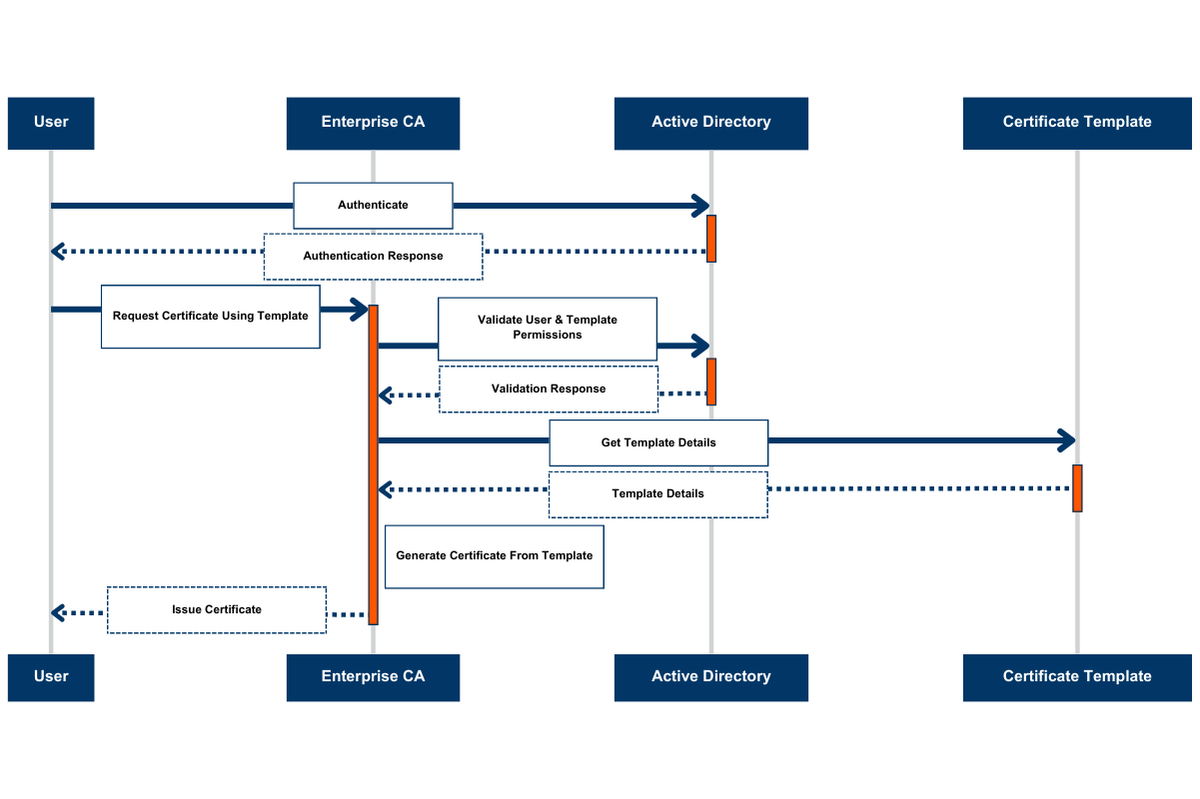
\includegraphics[width=0.75\linewidth]{cacert.png}
    \caption{FIGURE 4. User Enterprise Certificate Authority (CA) certificate retrieval workflow process}
    \label{fig:placeholder}
\end{figure}

In other words, AD CS sits at the core of enterprise identity trust. When configured correctly, it is a foundational pillar of security. When neglected, it becomes a silent but devastating avenue for compromise.

%\begin{table}[htbp]
\renewcommand{\arraystretch}{1.5}
\setlength{\tabcolsep}{8pt}
\rowcolors{3}{rowgray}{white}
\begin{tabular}{|p{3.5cm}|p{4.5cm}|p{5cm}|p{4cm}|}
\hline
\rowcolor{headerblue}
\multicolumn{4}{|l|}{\textcolor{white}{\textbf{TABLE 1: Recommendations Summary and Security Impact}}} \\

%\textbf{Area} & \textbf{Recommendation} & \textbf{Detail / Facts} & \textbf{Security Impact} \\
\hline
\textbf{SAN Configuration (Pre-KB5014754)} & \parbox[t]{4.5cm}{\begin{itemize}
    \item Disable use of custom SANs
    \item Require CA Manager approval
\end{itemize}} & \parbox[t]{5cm}{\begin{itemize}
    \item Templates allow manual SAN input
    \item Attackers can impersonate identities
\end{itemize}} & \parbox[t]{4cm}{\begin{itemize}
    \item Prevents identity spoofing
    \item Blocks unauthorized SAN issuance
\end{itemize}} \\
\hline
\end{tabular}




\begin{itemize}
    \item Templates allow manual SAN input
    \item Attackers can impersonate identities
\end{itemize} 
\begin{itemize}
    \item Prevents identity spoofing
    \item Blocks unauthorized SAN issuance
\end{itemize} 


\textbf{SAN Configuration (Post-KB5014754)} \\
\parbox[t]{4.5cm}{\begin{itemize}[leftmargin=*,nosep]
    \item Enforce CA Manager approval
    \item Disable custom SANs where allowed
\end{itemize} \\
\begin{tightitemize}
    \item Templates may still permit SAN input
    \item Default behavior may be insecure
\end{tightitemize} \\
\begin{tightitemize}
    \item Reduces attack surface
    \item Hardens post-patch certificate issuance
\end{tightitemize} \\
\hline

\textbf{CA Flags} \\
\begin{tightitemize}
    \item Remove \texttt{EDITF\_ATTRIB\_USE\_SUBJECT\_ALT\_NAME2}
\end{tightitemize} \\
\begin{tightitemize}
    \item Flag enables SAN injection from requests
    \item Often left enabled by default
\end{tightitemize} \\
\begin{tightitemize}
    \item Prevents crafted request abuse
    \item Ensures stronger identity control
\end{tightitemize} \\
\hline

\textbf{Template Permissions} \\
\begin{tightitemize}
    \item Restrict enrollment to known users/groups
    \item Audit template ACLs
\end{tightitemize} \\ 
\begin{tightitemize}
    \item Overly broad permissions common
    \item Risk of privilege escalation
\end{tightitemize} \\
\begin{tightitemize}
    \item Limits lateral movement
    \item Aligns with least privilege
\end{tightitemize} \\
\hline

\textbf{Template Review} & 
\begin{tightitemize}
    \item Review templates with domain-auth EKUs
\end{tightitemize} \\\& 
\begin{tightitemize}
    \item Some templates allow domain auth by default
    \item EKUs may be improperly assigned
\end{tightitemize} \\\& 
\begin{tightitemize}
    \item Prevents unauthorized domain authentication
    \item Strengthens PKI integrity
\end{tightitemize} \\
\hline

\textbf{CA Hierarchy} \\\& 
\begin{tightitemize}
    \item Treat Root/Sub CAs as Tier 0 assets
    \item Restrict logon access
\end{tightitemize} \\\& 
\begin{tightitemize}
    \item CA servers are high-value targets
    \item Often exposed to broader access
\end{tightitemize} \\\& 
\begin{tightitemize}
    \item Protects trust boundary
    \item Reduces risk of full PKI compromise
\end{tightitemize} \\
\hline

%\end{tabular}
\caption{Summary of recommendations with details and their security impacts}
%\end{table}


****************************************************

\begin{table}[htbp]
\centering
\centering
\caption{Certificate Mapping Hardening}
\begin{tabular}{|p{3.5cm}|p{6cm}|p{6cm}|}
\hline
\rowcolor{headerblue}
\multicolumn{3}{|l|}{\textcolor{white}{\textbf{TABLE 1: KB5014754-Strong Certificate Mapping Hardening}}} \\
\hline
\\textbf{Area} \\\& \textbf{Recommendation} \\\& \textbf{Detail / Facts} \\
\hline

\textbf{KB5014754 Update} \\\& 
\begin{compactitem}
    \item Installation of KB5014754 with full enforcement of Strong Certificate Mappings
    \item Audit and reduce \textit{Enroll / Auto-enroll} rights on certificate templates
    \item Ensure only authorized security groups (e.g., Domain Computers, specific service accounts) have access
\end{compactitem} \\\& 
\begin{compactitem}
    \item Released May 2022, enforced November 2022
    \item Ensures strict mapping of SAN/Subject fields to the actual AD account
    \item Prevents ambiguous or weak mappings
\end{compactitem} 
\begin{compactitem}
    \item Blocks abuse of misissued certificates used in AD CS privilege escalation (ESC1/ESC2/ESC3)
\end{compactitem} \\
\hline

\textbf{CA Flag: \texttt{EDITF\_ATTRIBUTESUBJECTNAME2}} \\\& 
\begin{compactitem}
    \item Remove this flag from all CAs where enabled
    \item Shorten certificate lifetimes for user and service templates (e.g., 1 year instead of 5)
    \item Reduce the persistence window if a malicious certificate is issued
    \item Force re-issuance under hardened rules after KB5014754 enforcement
\end{compactitem} \\\& 
\begin{compactitem}
    \item This flag permits requestors to insert arbitrary SANs into certificates. Microsoft recommends removing unless business-critical.
\end{compactitem} 
\begin{compactitem}
    \item Prevents attackers from issuing certificates that impersonate privileged accounts (e.g., Domain Admins)
\end{compactitem} \\
\hline

\textbf{Certificate Templates-Custom SANs} \\\& 
\begin{compactitem}
    \item Disable the use of custom SANs on all templates
    \item Review who can act as an Enrollment Agent and limit this to trusted security groups only
    \item Enforce multi-party approval or additional monitoring for any Enrollment Agent usage
    \item Regularly audit Enrollment Agent templates and revoke unused or unnecessary assignments
\end{compactitem} \\\& 
\begin{compactitem}
    \item Templates allowing user-defined SAN values enable attackers to request certificates with forged UPNs or DNS names.
\end{compactitem} 
\begin{compactitem}
    \item Eliminates common AD CS abuse vectors, for example, ESC1 in Certify / Certipy).
\end{compactitem}
\hline

\textbf{CA Manager Approval} \\\& 
\begin{compactitem}
    \item Enforce "CA Certificate Manager Approval" for any template supporting SANs enrollment to known users/groups
    \item Apply approval requirements only to high-risk templates
    %\item Identify all certificate templates that allow Subject Alternative Names (SANs) and configure them to require explicit CA Manager approval before issuance
    \item Ensures oversight is focused on templates most likely to be abused
\end{compactitem}

    \item Requires manual approval before issuance of certificates with SANs.
    \item Provides oversight and governance.
\begin{compactitem}
    \item Adds visibility and reduces the risk of stealthy certificate-based privilege escalation.
\end{compactitem} \\
\hline

\textbf{Monitoring and Visibility} \\\& 
\begin{compactitem}
    \item Configure advanced audit policies to capture certificate template changes, CA flag modifications, and certificate issuance events
    \item Ensure relevant security Event IDS (4886-4889 for template / CA changes, 4887 for issuance) are logged consistently
    \item Forward CA logs and Security event logs to a SIEM or log aggregator
\end{compactitem} \\\& 
\begin{compactitem}
    \item Use Event ID 4887 (certificate issued)
    \item Use Event IDs 4898 and 4899 (template changes)
    \item Configure SIEM alerts
\end{compactitem} 
\begin{compactitem}
    \item Detects attempts to enable SAN abuse or anomalous certificate enrollment activities.
\end{compactitem} \\
\hline

\textbf{Certificate Revocation and Recovery} \\\& 
\begin{compactitem}
    \item Implement CRL / OCSP Monitoring and Rapid Revocation Procedures
    \item Implement Role-Based Access Control (RBAC) for CA Administrators and define and enforce separate administrative roles (CA Managers, certificate publishers, auditors)
    \item Harden CA server configurations by applying relevant security benchmarks, baselines, STIGs, and SRGs
    \item Run the CA on a dedicated, hardened server that follows Tier 0 isolation principles
    \item Disable unnecessary services, restrict network access, and ensure the CA is patched regularly
    \item Scope certificate templates to specific security groups only instead of default "Authenticated Users"
\end{compactitem} \\\& 
\begin{compactitem}
    \item Ensure Certificate Revocation Lists (CRLs) and Online Certificate Status Protocol (OCSP) responders are operational, accessible, and monitored
    \item Document and test rapid revocation workflows for compromised or misissued certificates
\end{compactitem} 
\begin{compactitem}
    \item Provides the ability to quickly invalidate abused certificates
    \item Limits persistence of attacker-issued credentials
    \item Strengthens overall trust in PKI
\end{compactitem} \\
\hline

\end{tabular}
\caption{Summary of recommendations with details and their security impacts}
\end{table}

\section{Common Abuse Scenarios-Subject Alternative Names (SPNs)}
Active Directory Certificate Services (AD CS) provides organizations with the ability to use certificate-based authentication for both users and machines. This is often leveraged in protocols such as Kerberos (for user / service authentication) and the \textit{Secure Channel}(\texttt{netlogon)} protocol (for machine authentication).

\subsection{AD CS Domain Controller Certificate Verification and Validation Process}
When a certificate is presented to a Domain Controller (DC) during the authentication process, the DC performs several verification and validation checks before finally granting access. These checks include:
\subsubsection{1. Certificate Validity}
The DC ensures that the certificate was issued by a trusted Certificate Authority (CA) within the environment and that it falls within the defined validity period.
\subsubsection{2. Revocation Status}
The DC then confirms that the certificate has not been revoked via the Certificate Revocation List (CRL) or the Online Certificate Status Protocol (OCSP).
\subsubsection{3. Identity Mapping}
The DC attempts to correlate the certificate to an Active Directory account. This mapping process determines "who" the certificate represents within the domain.

\subsection{Certificate Mapping in Active Directory}
The certificate mapping is the mechanism that links a presented certificate to a specific AD account. There are two primary mapping methods that exist:
\subsubsection{1. Implicit Mapping}
\begin{itemize}
    \item The certificate is mapped automatically by AD, using values present in the certificate's Subject Alternative Name (SAN) field (such as a User Principal Name [UPN] or DNS host name).
    \item This is the most common mapping scenario in environments with auto-enrollment templates.
\end{itemize}
\subsubsection{2. Explicit Mapping}
\begin{itemize}
    \item An administrator deliberately associates a certificate with an account by writing its identity into the account's \texttt{altSecurityIdentities} attribute.
    \item This method is more controlled, but requires manual configurations and maintenance.
\end{itemize}

\subsection{The Role of SANs in Abuse}
By default, most certificate templates in AD CS are designed to populate the Subject and SAN fields automatically with values already present in Active Directory (e.g., the user's UPN or the computer's DNS host name). This ensures that a certificate accurately represents the requesting identity, and is not an impersonation, or fraudulent attempt.

However, certain templates can be configured with the option \textit{"Supply in the request."} When enabled, this setting allows the requestor to explicitly specify custom SAN values directly in the certificate signing request (CSR).

This, in turn, introduces a very dangerous attack surface.

First, any user with enrollment rights to a template can craft a CSR that includes arbitrary SAN entries, such as the UPN of a highly privileged account such as Domain Administrators, for example.

Second, if the template supports client authentication and does not require manual CA manager approval, the CA will proceed with issuing the certificate without any further verification or validation checks.

Finally, when presented to the Domain Controller, the certificate will authenticate as the privileged account named in the SAN-not the low-privilege account that requested it.

\section{Abuse Path and Privilege Escalation}
This misconfiguration opens the door to a classic privilege escalation pathway within Active Directory. The sequence begins when a low-privilege domain user identifies a certificate template that has been configured to allow the Subject Alternative Name (SAN) to be supplied in the certificate request. Unlike standard templates that automatically populate the SAN from Active Directory attributes, this setting allows the requestor to specify specific custom values.

Armed with this capability, the attacker generates a Certificate Signing Request (CSR) containing a forged User Principal Name (UPN). Instead of using their own UPN, the attacker substitutes the UPN of a highly privileged account, such as a Domain Administrator. From the perspective of the Certification Authority (CA), there is no distinction between legitimate and fraudulent SAN values if no approval process is enforced. The CA dutifully issues a certificate that includes the maliciously crafted SAN, effectively vouching for the attacker's claim of identity.

Once issued, the attacker presents this forged certificate during authentication. The Domain Controller receives the certificate, verifies that it was signed by a trusted CA and remains within its validity period, and then proceeds to map the identity. Because the certificate contains the UPN of the privileged account, the Domain Controller will interpret the authentication attempt as originating from that high-value identity. In this way, the attacker's low-privilege account is bypassed entirely, and authentication succeeds as though the attacker were the Domain Admin account itself.

The end result is that the attacker has escalated from a standard domain user to possessing full administrative control of the domain. Critically, this attack bypasses password-based controls altogether. Even if the targeted privileged account rotates its password, the rogue certificate remains valid until its expiration data or revocation, allowing persistent unauthorized backdoor access.

When combined with auto-enrollment, where the CA issues certificates automatically without requiring manual approval, the attack becomes nearly trivial to execute because any authenticated user who can essentially request certificates from such a template has a direct path from unprivileged access to complete domain compromise, with minimal effort and a high degree of stealth.
A high-level overview of this attack path is depicted in Figure 1.
\begin{figure}
    \centering
    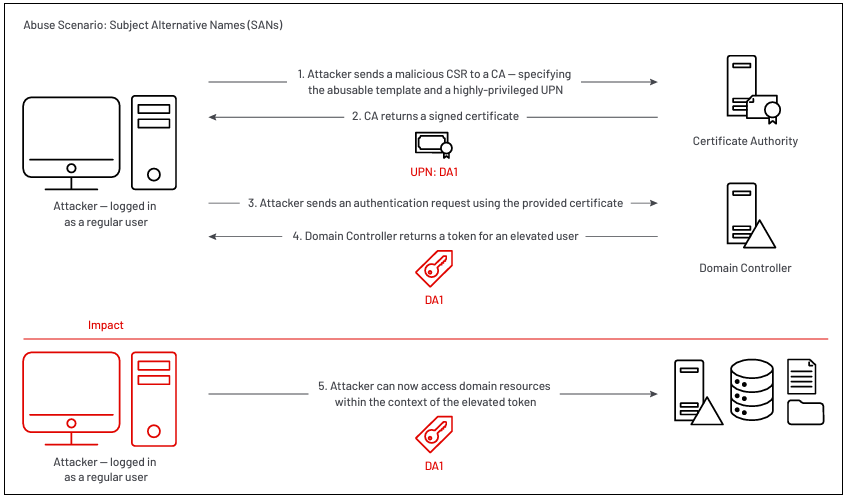
\includegraphics[width=0.75\linewidth]{sanattack.png}
    \caption{\textbf{FIGURE 1.} Attack path example of SAN abuse for privilege escalation}
    \label{fig:placeholder}
\end{figure}

\section{Golden Certificate Attack}
Within Active Directory environments, Certificate Services play a critical role in establishing trust. As part of the standard Public Key Infrastructure (PKI) process, a Certificate Authority (CA) is responsible for issuing certificates to users, computers, and services. When a user or machine submits a Certificate Signing Request (CSR), the CA verifies and validates that the request is valid and then signs the resulting certificate with its own private key. This signed certificate can be used later within Active Directory to authenticate identities, establish secure communications, and prove the legitimacy of the requesting entity. The integrity of this process depends entirely on the secrecy of the CAs private key, because the Domain Controllers rely on the corresponding CA public certificate to validate issued certificates.

By design, the CAs private key is protected to prevent misuse and abuse. Windows leverages the \textit{Data Protection API (DPAPI)} to protect this key. DPAPI uses a symmetric key derived from the CA server's local computer account credentials to encrypt the private key material, making it accessible only within the context of that machine. In practice, however, the private key is marked as exportable, meaning that anyone with sufficient local privileges on the CA server can extract it. Local administrators, for example, can use the \textit{Certificate Services Management Console (MMC)} to export the key directly, or they can turn to post-exploitation tools such as Mimikatz, SharpDPAPI, or \texttt{certutil.exe} to recover it in plaintext form.

Once an attacker compromises the CA server and successfully extracts the CA private key, the security of the entire PKI infrastructure-and, therefore, the Active Directory forest-is fundamentally broken. With the private key in hand, the adversary is no longer restricted to operating within the AD CS infrastructure. They can forge and sign certificates completely offline, issuing themselves certificates for any identity they choose without ever contacting the CA again. These malicious certificates are indistinguishable from legitimate ones because they are signed with the trusted CAs valid key.

The implications of this cyberattack are severe. An attacker can impersonate any account in the domain or forest, including highly privileged identities such as Domain Administrators, Schema Administrators, Backup Operators, Enterprise Admins, or even service accounts tied to critical Tier 0 systems. Unlike password theft, this compromise is extraordinarily durable. Certificates issued with the stolen key remain valid until the CAs own certificate expires or is revoked. Even if defenders rotate passwords, reset Kerberos tickets, or replace account credentials, the attacker's forged certificates will continue to authenticate as legitimate accounts until the root of trust itself is rebuilt from the ground up.

Equally dangerous is the fact that this malicious issuance process can be carried out entirely offline! Because the attacker no longer requires access to the CA server or AD CS infrastructure once the key has been stolen, their activities produce no logs, no enrollment events, and no traceable artifacts within Active Directory. Traditional detection mechanisms, such as monitoring for unusual template enrollment or certificate-issuance events, are completely bypassed. Defenders may not realize the compromise until long after persistence has been established.

This technique, commonly referred to as the \textit{Golden Certificate attack,} is conceptually similar to the \textit{Golden Ticket attack,} where attackers forge Kerberos tickets offline using the \texttt{krbtgt} account key. In both cases, the adversary has compromised the cryptographic root of trust-the key material that allows them to mint arbitrary credentials with complete legitimacy in the eyes of AD and the DCs. The difference is that while Golden Tickets rely on Kerberos trust, Golden Certificates exploit the PKI trust chain, often giving attackers stealthier, longer-lasting, and harder-to-detect access.

In summary, compromise of a CA private key enables adversaries to subvert the entire authentication fabric of Active Directory. With the ability to forge Golden Certificates, attackers gain virtually unlimited persistence, full impersonation capabilities, and the means to bypass even the most rigorous password and ticketing hygiene. The only effective recovery is a complete reestablishment of trust, which typically requires rebuilding the PKI from scratch-a disruptive, resource-intensive, and high-impact process for any defender and enterprise.

\begin{figure}
    \centering
    
    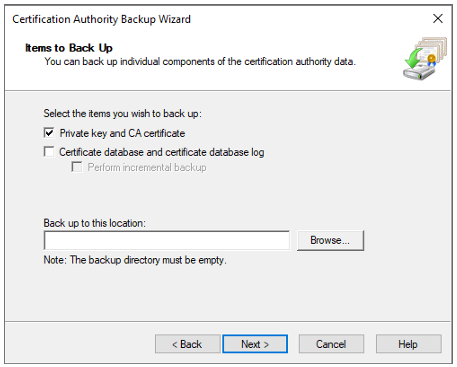
\includegraphics[width=0.75\linewidth]{cabackup.png}
    \caption{\textbf{FIGURE 2.} MMC method to backup a CAs private key and certificate}
    \label{fig:placeholder}

\end{figure}

\section{Template Permissions}
Certificate templates are foundational components within Active Directory Certificate Services (AD CS), defining the rules and attributes that govern how certificates are issued. These templates, like all Active Directory objects, are governed by \textit{security descriptors.}A security descriptor is essentially an Access Control List (ACL) that specifies which security principals-users, groups, or computers-are authorized to interact with the object and what specific operations they are permitted to perform. \textit{Access Control Entries (ACEs),} within the descriptor determine these rights, ranging from the ability to enroll for certificates, to more sensitive permissions such as modifying template properties.

\subsection{Template Permissions in Practice}
In secure deployments, certificate template permissions are carefully locked down so that only administrators or tightly scoped groups have the ability to manage them. This prevents abuse of the certificate issuance process; however, in real-world environments, I have repeatedly encountered situations where certificate templates were configured with overly permissive Access Control Entries (ACEs).

During one CCRI (Cyber Command Readiness Inspection), my role was to assume the identity of a regular, non-privileged domain user. The objective was simple: determine how far I could push access inside the network perimeter starting from the same position an average employee might hold. The initial focus was on external-facing DoD systems-WiFi, perimeter firewalls, and edge routers-but once I pivoted internally, I began enumerating Active Directory Certificate Services (AD CS) with my trusty little "hacking" journal in hand.

\begin{figure}
    \centering
    
\includegraphics[width=1\linewidth,height=0.7\textheight,keepaspectratio]{me1.png}
    \caption{FIGURE Me and my trusty little hacking journal}
    \label{fig:placeholder}
\end{figure}

To my surprise, within just a couple of hours, I identified a certificate template that I, as a low-privileged user, had the ability to modify. The sensitive properties exposed in this template included enrollment rights, issuance requirements, and, critically, flags that controlled how certificate subjects and SANs were defined. Being able to change these properties gave me a direct pathway to increasing my privileges. In other words, what should have been a tightly controlled security object was left wide open, and that misconfiguration provided me with an \textit{open door into the organization's crown jewels.} I was queen of the castle (well, a portion of it, to say the least).

Now, it is important to state the need for understanding the mindset of an attacker-an attacker who lives and breathes security exploitation. 24x7x365. Skilled adversaries (and defenders as well) study their target(s) environment obsessively. If they do not already know how to abuse a setting, they will exhaustively research it, digging into every available detail until they uncover the exact weakness they can exploit. This means that what defenders might view as a minor oversight-whether the result of a deliberate convenience choice or an accidental misconfiguration-such as an unnecessary permission or a poorly scoped ACL, can quickly become a fully weaponized attack vector in the hands of a motivated adversary.

This is precisely why permissions hygiene is so critical in any environment. Permissions act as gatekeepers of security; they are the unseen locks and barriers that literally prevent unauthorized users from slipping inside. Yet, all too often, permissions are treated as something that one may "set and forget." At the time an administrator creates them, it might feel like locking them down too tightly is inconvenient, unnecessary, or even counterproductive to productivity. But that momentary convenience evaporates instantly when a breach occurs. Once sensitive data are exposed or an attacker is able to move freely through systems because of loose or mismanaged permissions, suddenly the value of strict access control becomes painfully obvious. It is that feeling of having shot yourself in the foot. What once felt restrictive now seems like the most convenient and necessary safeguard imaginable.

An illustrative example highlights how dangerous these misconfigurations can be. Suppose a non-privileged user has the rights to enable the flag \texttt{\detokenize{CT_FLAG_ENROLLEE_SUPPLIES_SUBJECT_ALT_NAME}} on a certificate template. This single change grants the ability for requestors to insert custom Subject Alternative Names (SANs) into their certificate requests. From there, it is trivial for the attacker to submit a request containing the User Principal Name (UPN) of a domain administrator or other high value account. If the template also permits client authentication, the CA will happily issue a certificate mapped to that privileged identity. When presented to a Domain Controller, the forged certificate is accepted as legitimate, allowing the attacker to impersonate a domain administrator without ever knowing their password.

The consequences are profound: what began as an engagement with the rights of a standard user ended in a full domain compromise simply because of overly permissive template ACLs. This scenario really underscores the broader lesson here: that misconfigured permissions, regardless of where they may exist, can quickly transform strong defenses into trivial barriers for attackers to pummel through.

\subsection{How the Vulnerable Certificate Template Was Found}
As a non-privileged user on a penetration test, I was not expecting to stumble across flashy exploits right out of the gate-which almost never happens. Real penetration testing is about patience and persistence, not Hollywood-style instant wins. Effective threat hunting requires patience, methodical probing and prodding, and careful navigation through the domain carefully, methodically, and always with an eye toward avoiding detection. In any serious security engagement, you don't expect to find the big prize immediately. The real vulnerabilities, the ones that matter, take time, patience, and deliberate exploitation to uncover.

I started enumerating what was already available to me. Since certificate template permissions are often overlooked or lax, I began by enumerating certificate templates in the domain to see if I could come up with any accessible ones I could request.

The two primary tools for this type of enumeration that I used were Certutil (native to Windows) and, what I call, "C-Deuce," which is Certify (C\#) and Certipy.  Certify and Certipy are powerful tools that are used to penetrate Active Directory Certificate Services (AD CS) .

\subsubsection{Certify (C\#)}
Certify is a C# tool primarily used in Windows systems to attack and enumerate Active Directory Certificate Services (AD CS) environments. I features identification of PKI enrollment services, potential attack pathways, request of certificates, and performing enumeration operations. Certipy, on the other hand, is a Python-based toolkit that is also used to enumerate and abuse AD CS misconfigurations, including all known ESC1-ESC16 attack pathways.

\subsection{Did You Know?}
\textbf{The ESC1-ESC16 Abuse Paths in Active Directory Certificate Services (AD CS)}
Active Directory admins may feel they understand the privileged accounts that exist in their environment(s) and have adequately protected them; however, in many environments, Active Directory Certificate Services (AD CS) misconfigurations effectively give any user access to Domain Admins, regardless of what their account privilege is. This can undermine efforts to secure accounts and leave organizations vulnerable to widespread compromise as attackers escalate privileges and pivot across domains.

These misconfigurations are easy to make due to the complex nature of AD CS configuration-I regularly find at least one AD CS issue in customer engagements. In recent years, attackers have become more aware of these issues, making it more critical for administrators and defenders to understand \textit{all} the privilege escalation pathways in their domains and how to detect their active exploitation, to improve the security stances of Active Directory.

When security researchers talk about "ESC" paths in AD CS, they refer to a taxonomy of \textit{Exploitation Scenarios (ESC).} The exploitation of AD CS misconfigurations became a key concern when, in 2021, researchers at SpectreOps called attention to the problem in a whitepaper by Will Schroeder and Lee Christensen of SpectreOps titled, \textit{"Certified Pre-Owned."}  Because AD CS is used for authentication, these attacks pose a significant threat that carries severe consequences for organizations-including the potential for full domain compromise-making them a prime target for threat actors. To give defenders and security teams a better understanding of attackers and their TTPs, the ESC1-ESC16 were born. Each ESC scenario represents a distinct way in which adversaries can abuse misconfigurations or weak controls in AD CS to escalate privileges, persist, or impersonate accounts.

Think of ESC pathways as a catalog \textit{ of known attack techniques} against the Public Key Infrastructure (PKI) of the enterprise. If an attacker has a toehold in your environment, these are the likely avenues that they will test for privilege escalation or persistence. If you defend AD CS, these are the misconfigurations that you need to know, monitor, and eliminate.

The core driving force behind the creation of the ESC1-ESC16 classification system and the accompanying research (the "Certified Pre-Owned" whitepaper) was the increasing recognition and need to address the widespread and critical security vulnerabilities within AD CS. This research comprehensively details various techniques for attacking AD CS to achieve persistence, credential theft, and privilege escalation.

\subsection{Key Features of ESC Pathways}
1. Widespread Misconfigurations and Lack of Awareness:
Researchers and security practitioners observed that AD CS was frequently misconfigured, leading to easy pathways for privilege escalation within Active Directory environments. Many organizations were unaware of these vulnerabilities or lacked the expertise to properly secure their AD CS deployments.

2. Significant Impact of Exploitation:
Exploiting these misconfigurations can grant attackers highly privileged access, often leading to full domain compromise, including Domain Admin privileges. This presented a serious threat to organizational security.

3. Need for a Structured Approach:
Previously, knowledge about AD CS attacks was more fragmented. The SpectreOps team aimed to provide a comprehensive and systematic way to classify and explain these attack techniques. The "ESC" (Escalation) numbering system provides that structure.

4. Empowering Defenders and Red Teams:
By clearly describing the different misconfigurations, exploitation methods, and detection/mitigation strategies, the researchers sought to empower both defenders (blue teams) to identify and remediate vulnerabilities, and red teams / penetration testers to effectively assess the AD CS security posture.

5. Facilitating Tool Development:
The structured approach also paved the way for the creation of tools like Certify and Certipy, which automate the process of finding and, in some cases, exploiting these AD CS vulnerabilities, simplifying the assessment and remediation process.

\subsection{The Reason Behind the Creation of the ESC Attack Classifications}
The growing recognition of Active Directory (AD CS) vulnerabilities did not happen overnight. For years, penetration testers and red teamers had identified isolated weaknesses in certificate services, such as misconfigured templates or overly broad enrollment rights; however, there had never been a comprehensive body of research that tied all these attack paths together in a way that defenders could clearly understand. SpectreOps sought to change that. Their work consolidated scattered findings and expanded on them, demonstrating that AD CS misconfigurations represented a massive and often overlooked blind spot in enterprise security.

To bring order and clarity to these vulnerabilities, the researchers introduced a systematic classification model known as the ESC (Escalation) taxonomy. Each "ESC" number, from ESC1 to ESC16, represents a unique abuse scenario tied to AD CS infrastructure. This numbering system not only provides a common language for security professionals to discuss these attacks, but also highlighted the breadth of possible misconfigurations, ranging from template permissions to certificate authority flags and web enrollment services.

The impact of their research was striking. In almost every enterprise network SpectreOps analyzed, AD CS misconfigurations enabled privilege escalation. The findings showed that attackers starting with only low-level domain user rights could often leverage these flaws to gain control over entire Active Directory forests. What made this more alarming was the relative ease of exploitation-many techniques required no special privileges and left little trace within standard monitoring solutions.

To support both offensive and defensive teams, tool development went hand in hand with research. SpectreOps released \textbf{Certify}, a PowerShell-based toolkit designed to audit and exploit AD CS environments, making it easier to test for misconfigurations. Building on this, security researcher Oliver Lyak released \textbf{Certipy,} a Python-based port of Certify, which extended the functionality to non-Windows environments and became a staple in red team toolkits. Both tools, widely available on GitHub, have been instrumental in demonstrating real-world abuse cases and in helping defenders better identify weaknesses before adversaries do.

Together, this body of work-comprehensive research, the ESC taxonomy, and the release of practical tooling-transformed how the security community views Active Directory Certificate Services. What was once a niche area of PKI administration is now recognized as one of the most critical and exploitable attack surfaces in Active Directory.

\subsection{Precise Breakdown of the ESC1-ESC16 Taxonomy}
The ESC taxonomy is important because it gives both \textit{attackers} and \textit{defenders} a shared language to understand the risk of AD CS. From a red team perspective, ESC1-ESC8 are the \textbf{ most frequently} exploited in real-world engagements (misconfigured templates and NTLM relay). From a blue team perspective, knowing the taxonomy helps build detection and hardening strategies.
\begin{itemize}
    \item Audit for templates that allow SAN supply (ESC1).
    \item Lock down template permissions (ESC2, ESC5).
    \item Monitor CA flags such as \texttt{EDITF\_ATTRIBUTESUBJECTALTNAME2} (ESC7).
    \item Harden web enrollment endpoints to prevent NTLM relay (ESC8).
\end{itemize}

Ultimately, AD CS sits at the Tier 0 trust boundary of Active Directory. Any one of these misconfigurations can turn into a domain compromise if left unchecked.

Below is a precise breakdown of the 16 major ESC paths (simplified but detailed enough for readers to grasp):

\subsubsection{ESC1-Widespread Misconfigurations and Lack of Awareness (SAN Supply)}
Researchers and security practitioners observed that AD CS was frequently misconfigured, leading to easy pathways for privilege escalation within Active Directory environments. Many organizations were unaware of these vulnerabilities or lacked the expertise to properly secure their AD CS deployments.

\subsubsection{ESC2-Misconfigured Certificate Templates (Weak Permissions)}
\begin{itemize}
    \item Template ACLs grant low-privileged users the ability to modify settings.
    \item Attackers enable dangerous flags like SAN supply or client authentication.
\end{itemize}

\subsubsection{ESC3-Misconfigured Certificate Templates (Dangerous EKUs)}
\begin{itemize}
    \item Templates include Application Policies / Enhanced Key Usages (EKUs) such as \textit{Certificate Request Agent} or \textit{Any Purpose.}
    \item Attackers can use these certificates for unintended authentication scenarios.
\end{itemize}
% If you intended to center something here, use the center environment:


\subsubsection{ESC4-Certificate Enrollment Agent Abuse}
\begin{itemiz3
021e}
    \item Enrollment Agent templates allow a user to request certificates on behalf of other accounts.
    \item If the permissions are weak, an attacker can impersonate privileged users.
\end{itemize}

\subsubsection{ESC5-Misconfigured Certificate Templates (Enrollment Rights)}
\begin{itemize}
    \item Templates grant enrollment to overly broad groups such as Enterprise Admins, Schema Admins, or Domain Admins.
    \item Any user can register for certificates with sensitive EKUs or SANs.
\end{itemize}

\subsubsection{ESC6-Vulnerable Certificate Authority ACLs}
\begin{itemize}
    \item The ACLs of the CA object in AD are misconfigured.
    \item Attackers can directly modify CA settings, issue certificates, or grant themselves rights.
\end{itemize}

\subsubsection{ESC7-Misconfigured Certificate Authority \texttt{EDITF\_ATTRIBUTESUBJECTALTNAME2} Flag}
\begin{itemize}
    \item CA-level flag allows for arbitrary SANs in any certificate request.
    \item Attackers can impersonate privileged users even without template misconfigs.
\end{itemize}

\subsubsection{ESC8-NTLM Relay to AD CS (HTTP Enrollment Services)}
\begin{itemize}
    \item If Certificate Enrollment Web Services don't require signing or encryption, attackers can relay NTLM authentication to obtain a certificate as a victim user.
\end{itemize}

\subsubsection{ESC9-Cross-Forest Trust Abuse (Weak Mapping)}
\begin{itemize}
    \item Trusts between forests are based on weak identity mappings.
    \item Attackers forge certificates in one forest to gain access in another.
\end{itemize}

\subsubsection{ESC10-Enterprise Admin-to-CA Misconfiguration}
\begin{itemize}
    \item Enterprise Admins configure or delegate CA incorrectly.
    \item Attackers exploit permissions to issue backdoor certificates.
\end{itemize}

\subsubsection{ESC11-Weak PKI Infrastructure (Subordinate CA Abuse)}
\begin{itemize}
    \item Attackers compromise or leverage a misconfigured subordinate CA.
    \item This allows them to issue trusted certificates up the chain.
\end{itemize}

\subsubsection{ESC12-Offline Root CA Compromise}
\begin{itemize}
    \item The root CA key is compromised or not sufficiently protected.
    \item Attackers can issue trusted certificates for the entire enterprise.
\end{itemize}

\subsubsection{ESC13-Misconfigured Certificate Enrollment Web Services (CES / CEP)}
\begin{itemize}
    \item Weak authentication or permissions on enrollment services.
    \item Attackers abuse web-based enrollment to impersonate accounts.
\end{itemize}

\subsubsection{ESC14-Cross-Forest Misconfigurations (Enrollment Rights)}
\begin{itemize}
    \item Misconfigured enrollment rights extend across forest trusts.
    \item Attackers request certificates from foreign forests to escalate.
\end{itemize}

\subsubsection{ESC15-Certificate Services DACL Abuse (AD Objects)}
\begin{itemize}
    \item Attackers manipulate AD objects tied to certificate issuance, such as \texttt{NTAuthCertificates} or Public Key Services containers.
\end{itemize}

\subsubsection{ESC16-Abuse of Certificate Authority Configuration}
\begin{itemize}
    \item Direct manipulation of CA registry or configuration files.
    \item Attackers can alter issuance policies, EKUs, or enforcement settings.
\end{itemize}

\section{AD CS ESC1-ESC16 vs. MITRE ATT\&CK Framework}
\begin{itemize}
    \item \textbf{Origin:} Created by SpectreOps during their landmark investigation of Active Directory Certificate Services (AD CS).
    \item \textbf{Scope:} Focuses \textit{exclusively} on misconfigurations and abuse paths in AD CS (enterprise PKI inside Active Directory).
    \item \textbf{Format:} A taxonomy of 16 specific scenarios (ESC1 through ESC16) that describe concrete misconfigurations, such as: \begin{itemize}
        \item ESC1: Templates that allow custom Subject Alternative Names (SANs).
        \item ESC7: Dangerous CA Flag \texttt{EDITF\_ATTRIBUTESUBJECTALTNAME2} enabled.
        \item ESC8: NTLM communication with web enrollment services.
    \end{itemize}
\item \textbf{Use Case:} Primarily for Active Directory / PKI defenders and red teamers. It is a \textit{niche, deep-dive framework} to understand how AD CS can be abused for privilege escalation and persistence.
\item \textbf{Output:} Gives you a checklist of AD CS-specific risks to audit and harden.
\end{itemize}

\subsection{MITRE ATT\&CK}
\begin{itemize}
    \item \textbf{Origin:} Developed and maintained by MITRE, a nonprofit that supports the US government.
    \item \textbf{Scope:} A global knowledge base of adversarial tactics, techniques, and procedures (TTPs) in \textit{ all domains -} Windows, Linux, Cloud, ICS, Mobile, and more.
    \item \textbf{Format:} Organized by \textit{Tactics} (the "why," like Persistence or Privilege Escalation) and \textit{Techniques/Subtechniques} (the "how," such as Pass-the-Ticket (PtT), Kerberoasting or Credential Dumping).
    \item \textbf{Use Case:} Used for threat modeling, detection engineering, red and blue team exercises, and incident response. Provides a standardized language to describe adversary behaviors at a high level.
    \item \textbf{Output:} Helps organizations align defenses and detections to known adversary behaviors throughout the kill chain.
\end{itemize}

\begin{table}[htbp]
\renewcommand{\arraystretch}{1.5}
\setlength{\tabcolsep}{8pt}
\rowcolors{3}{rowgray}{white}
\begin{tabular}{|p{3.5cm}|p{4.5cm}|p{5cm}|p{4cm}|}
\hline
\rowcolor{headerblue}
\multicolumn{4}{|l|}{\textcolor{white}{\textbf{TABLE 2: Key Differences- ESC vs. ATT\&CK}}} \\
\hline
\textbf{Aspect} \\\& \textbf{ESC1-ESC16} \\\& \textbf{MITRE ATT\&CK} \\
\hline

\textbf{Focus} \\\& 
\begin{compactitem}
    \item Narrow: AD CS misconfigurations and abuse
\end{compactitem} \\\& 
\begin{compactitem}
    \item Broad: Adversary behaviors across all domains
\end{compactitem} \\
\hline

\textbf{Granularity} \\\& 
\begin{compactitem}
    \item Very specific (certificate templates, CA flags, AD CS abuse)
\end{compactitem} \\\& 
\begin{compactitem}
    \item More granular (techniques applicable across many technologies)
\end{compactitem} \\
\hline

\textbf{Purpose} \\\& 
\begin{compactitem}
    \item Educate defenders about PKI / AD CS risks
    \item Guide red team exploitation
\end{compactitem} \\\& 
\begin{compactitem}
    \item Provide universal framework for adversary behavior, detection, and defense
\end{compactitem} \\
\hline

\textbf{Creators} \\\& 
\begin{compactitem}
    \item SpectreOps (red team research organization)
\end{compactitem} \\\& 
\begin{compactitem}
    \item MITRE (U.S. government-backed research organization)
\end{compactitem} \\
\hline

\textbf{Use Case} \\\& 
\begin{compactitem}
    \item Checklist for AD CS hardening, pentests, audits
\end{compactitem} \\\& 
\begin{compactitem}
    \item Threat modeling, ATT\&CK mapping, SOC / DFIR detection engineering
\end{compactitem} \\
\hline
\end{tabular}
\caption{Summary of key differences between the ESC taxonomy and the MITRE ATT\&CK framework}
\end{table}

\tipbox{How They Relate
\begin{itemize}
    \item ESC1-ESC16 can be thought of as a specialized subset of techniques that fit inside the MITRE ATT\&CK framework under categories such as \textit{Credential Access, Persistence,} and \textit{Privilege Escalation.}
    \item For example:
        \item ESC1 (abusing SANs for impersonation) could map to MITREs T1552.001-Credentials in Certificates.
        \item ESC8 (NTLM relay to AD CS) could map to T1557-Adversary-in-the-Middle.
    \item But MITRE ATT\&CK does not go into the granular PKI/AD CS detail that ESC1-ESC16 does.
\end{itemize}}



One illustrative example is the ability for a non-privileged user to enable the flag \textbf{\texttt{CT_FLAG_ENROLLEE_SUPPLIES_SUBJECT_ALT_NAME}}, which permits requestors to supply custom Subject Alternative Names (SANs) in certificate requests. When this flag is enabled, an attacker can submit a certificate request with a forged SAN, such as the User Principal Name (UPN) of a Domain Admin account. If the template also supports client authentication, the CA will issue a certificate that effectively impersonates the privileged account, thereby enabling the attacker to escalate their privileges dramatically.